% Nguon SGK: trang 24--25, direct images trong issue #6.
% Nguon SBT: "SBT TOAN 9 KNTT TAP 1.pdf", trang 17--19,
% SHA-256 theo issue: d7ffd04618456682795977e5c47de7874161a35e8606e5bac1906881603a72f7.

\section*{Bài tập cuối chương I}

\begin{exercises}
    \subsection{Bài tập cuối chương I}

    \textbf{A. TRẮC NGHIỆM}

    \begin{questions}[resume=SGK]
        \item Cặp số nào sau đây là nghiệm của hệ phương trình
        \[
            \left\{
            \begin{aligned}
                5x+7y&=-1,\\
                3x+2y&=-5?
            \end{aligned}
            \right.
        \]
        \begin{tasks}(4)
            \task $(-1;1)$.
            \task $(-3;2)$.
            \task $(2;-3)$.
            \task $(5;5)$.
        \end{tasks}
        \par\noindent\answerbox\par

        \item Trên mặt phẳng tọa độ $Oxy$, cho các điểm $A(1;2)$, $B(5;6)$, $C(2;3)$, $D(-1;-1)$. Đường thẳng $4x-3y=-1$ đi qua hai điểm nào trong các điểm đã cho?
        \begin{tasks}(4)
            \task $A$ và $B$.
            \task $B$ và $C$.
            \task $C$ và $D$.
            \task $D$ và $A$.
        \end{tasks}
        \par\noindent\answerbox\par

        \item Hệ phương trình
        \[
            \left\{
            \begin{aligned}
                1{,}5x-0{,}6y&=0{,}3,\\
                -2x+y&=-2
            \end{aligned}
            \right.
        \]
        \begin{tasks}(2)
            \task Có nghiệm là $(0;-0{,}5)$.
            \task Có nghiệm là $(1;0)$.
            \task Có nghiệm là $(-3;-8)$.
            \task Vô nghiệm.
        \end{tasks}
        \par\noindent\answerbox\par

        \item Hệ phương trình
        \[
            \left\{
            \begin{aligned}
                0{,}6x+0{,}3y&=1{,}8,\\
                2x+y&=-6
            \end{aligned}
            \right.
        \]
        \begin{tasks}(2)
            \task Có một nghiệm.
            \task Vô nghiệm.
            \task Có vô số nghiệm.
            \task Có hai nghiệm.
        \end{tasks}
        \par\noindent\answerbox\par
    \end{questions}

    \textbf{B. TỰ LUẬN}

    \begin{questions}[resume=SGK]
        \item Giải các hệ phương trình:
        \begin{questions}
            \item $\left\{
                \begin{aligned}
                    2x+5y&=10,\\
                    \dfrac{2}{5}x+y&=1;
                \end{aligned}
                \right.$

            \answerline
            \answerline

            \item $\left\{
                \begin{aligned}
                    0{,}2x+0{,}1y&=0{,}3,\\
                    3x+y&=5;
                \end{aligned}
                \right.$

            \answerline
            \answerline

            \item $\left\{
                \begin{aligned}
                    \dfrac{3}{2}x-y&=\dfrac{1}{2},\\
                    6x-4y&=2.
                \end{aligned}
                \right.$

            \answerline
            \answerline
        \end{questions}

        \item Giải các hệ phương trình:
        \begin{questions}
            \item $\left\{
                \begin{aligned}
                    0{,}5x+2y&=-2{,}5,\\
                    0{,}7x-3y&=8{,}1;
                \end{aligned}
                \right.$

            \answerline
            \answerline

            \item $\left\{
                \begin{aligned}
                    5x-3y&=-2,\\
                    14x+8y&=19;
                \end{aligned}
                \right.$

            \answerline
            \answerline

            \item $\left\{
                \begin{aligned}
                    2(x-2)+3(1+y)&=-2,\\
                    3(x-2)-2(1+y)&=-3.
                \end{aligned}
                \right.$

            \answerline
            \answerline
        \end{questions}

        \item Tìm số tự nhiên $n$ có hai chữ số, biết rằng nếu viết thêm chữ số $3$ vào giữa hai chữ số của số $n$ thì được một số lớn hơn số $n$ là $585$ đơn vị, và nếu viết hai chữ số của số $n$ theo thứ tự ngược lại thì được một số nhỏ hơn số $n$ là $18$ đơn vị.

        \answerline
        \answerline
        \answerline

        \item Trên cánh đồng có diện tích $160$ ha của một đơn vị sản xuất, người ta dành $60$ ha để cấy thí điểm giống lúa mới, còn lại vẫn cấy giống lúa cũ. Khi thu hoạch, đầu tiên người ta cắt $8$ ha giống lúa cũ và $7$ ha giống lúa mới để đối chứng. Kết quả là, $7$ ha giống lúa mới cho thu hoạch nhiều hơn $8$ ha giống lúa cũ là $2$ tấn thóc. Biết rằng tổng số thóc (cả hai giống) thu hoạch cả vụ trên $160$ ha là $860$ tấn. Hỏi năng suất của mỗi giống lúa trên $1$ ha là bao nhiêu tấn thóc?

        \answerline
        \answerline
        \answerline

        \item Hai vật chuyển động đều trên một đường tròn đường kính $20$ cm, xuất phát cùng một lúc, từ cùng một điểm. Nếu chuyển động ngược chiều thì cứ sau $4$ giây chúng lại gặp nhau. Nếu chuyển động cùng chiều thì cứ sau $20$ giây chúng lại gặp nhau. Tính vận tốc (cm/s) của mỗi vật.

        \answerline
        \answerline
        \answerline

        \item Một người mua hai loại hàng và phải trả tổng cộng là $21{,}7$ triệu đồng, kể cả thuế giá trị gia tăng (VAT) với mức $10\%$ đối với loại hàng thứ nhất và $8\%$ đối với loại hàng thứ hai. Nếu thuế VAT là $9\%$ đối với cả hai loại hàng thì người đó phải trả tổng cộng $21{,}8$ triệu đồng. Hỏi nếu không kể thuế VAT thì người đó phải trả bao nhiêu tiền cho mỗi loại hàng?

        \answerline
        \answerline
        \answerline
    \end{questions}
\end{exercises}

\begin{practice}
    \subsection{Ôn tập chương I}

    \textbf{A. CÂU HỎI (Trắc nghiệm)}

    \begin{enumerate}
        \item Hệ phương trình nào sau đây là hệ hai phương trình bậc nhất hai ẩn?
        \begin{tasks}(2)
            \task $\left\{\begin{aligned}2x+y&=3\\x-z&=-1.\end{aligned}\right.$
            \task $\left\{\begin{aligned}2x+y&=3\\0x+0y&=1.\end{aligned}\right.$
            \task $\left\{\begin{aligned}2x+y&=3\\0x-y&=-1.\end{aligned}\right.$
            \task $\left\{\begin{aligned}2x+y&=3\\x+y^2&=1.\end{aligned}\right.$
        \end{tasks}
        \par\noindent\answerbox\par

        \item Nghiệm của hệ phương trình
        $\left\{\begin{aligned}4x+3y&=-1\\2x-y&=7\end{aligned}\right.$ là
        \begin{tasks}(4)
            \task $(-1;1)$.
            \task $(3;-1)$.
            \task $\left(\dfrac{1}{2};-1\right)$.
            \task $(2;-3)$.
        \end{tasks}
        \par\noindent\answerbox\par

        \item Trong mặt phẳng tọa độ $Oxy$, cho các điểm $M(1;2)$, $N(2;3)$, $P(-1;-1)$, $Q(5;8)$. Đường thẳng $3x-2y=-1$ đi qua hai điểm nào trong các điểm đã cho?
        \begin{tasks}(4)
            \task $M$ và $N$.
            \task $M$ và $P$.
            \task $P$ và $Q$.
            \task $N$ và $P$.
        \end{tasks}
        \par\noindent\answerbox\par

        \item Giá trị của $a$ và $b$ để đường thẳng $y=ax+b$ đi qua hai điểm $(1;-1)$ và $(-1;5)$ là
        \begin{tasks}(4)
            \task $a=1$, $b=-2$.
            \task $a=-5$, $b=1$.
            \task $a=-3$, $b=2$.
            \task $a=-1$, $b=0$.
        \end{tasks}
        \par\noindent\answerbox\par

        \item Hệ phương trình nào sau đây có nghiệm duy nhất?
        \begin{tasks}(2)
            \task $\left\{\begin{aligned}x-2y&=3\\2x-4y&=5.\end{aligned}\right.$
            \task $\left\{\begin{aligned}x-2y&=3\\-2x+4y&=-6.\end{aligned}\right.$
            \task $\left\{\begin{aligned}x-2y&=3\\2x+4y&=5.\end{aligned}\right.$
            \task $\left\{\begin{aligned}x-2y&=3\\-x+2y&=-2.\end{aligned}\right.$
        \end{tasks}
        \par\noindent\answerbox\par

        \item Hình bên dưới minh hoạ tập nghiệm của hệ phương trình nào sau đây?
        \begin{tasks}(2)
            \task $\left\{\begin{aligned}x-y&=1\\x-y&=3.\end{aligned}\right.$
            \task $\left\{\begin{aligned}x-y&=1\\x+y&=3.\end{aligned}\right.$
            \task $\left\{\begin{aligned}x+y&=1\\x-y&=3.\end{aligned}\right.$
            \task $\left\{\begin{aligned}x+y&=1\\x+y&=3.\end{aligned}\right.$
        \end{tasks}

        \begin{center}
            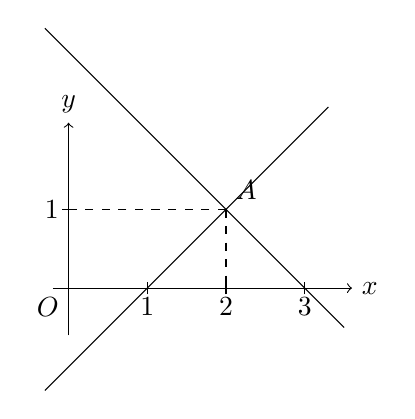
\begin{tikzpicture}
                \coordinate (O) at (0,0);
                \coordinate (A) at (2,1);
                \coordinate (Xone) at (1,0);
                \coordinate (Xthree) at (3,0);

                \draw[->] (-0.2,0) -- (3.6,0) node[right] {$x$};
                \draw[->] (0,-0.6) -- (0,2.1) node[above] {$y$};
                \draw (-0.08,1) -- (0.08,1);
                \draw (1,-0.08) -- (1,0.08);
                \draw (2,-0.08) -- (2,0.08);
                \draw (3,-0.08) -- (3,0.08);
                \node[below left] at (O) {$O$};
                \node[below] at (Xone) {$1$};
                \node[below] at (2,0) {$2$};
                \node[below] at (Xthree) {$3$};
                \node[left] at (0,1) {$1$};

                \draw (-0.3,-1.3) -- (3.3,2.3);
                \draw (-0.3,3.3) -- (3.5,-0.5);
                \draw[dashed] (A) -- (2,0);
                \draw[dashed] (A) -- (0,1);
                \node[above right] at (A) {$A$};
            \end{tikzpicture}
        \end{center}
        \par\noindent\answerbox\par

        \item Hệ phương trình $\left\{\begin{aligned}3x-ay&=b\\ax+by&=3\end{aligned}\right.$ có nghiệm là $(2;-3)$ khi
        \begin{tasks}(4)
            \task $a=3$, $b=3$.
            \task $a=3$, $b=-3$.
            \task $a=-3$, $b=3$.
            \task $a=-3$, $b=-3$.
        \end{tasks}
        \par\noindent\answerbox\par

        \item Hệ phương trình $\left\{\begin{aligned}x+my&=1\\-mx-y&=-1\end{aligned}\right.$ có vô số nghiệm trong trường hợp nào sau đây?
        \begin{tasks}(4)
            \task $m=1$.
            \task $m=-1$.
            \task $m=2$.
            \task $m=-2$.
        \end{tasks}
        \par\noindent\answerbox\par
    \end{enumerate}

    \textbf{B. BÀI TẬP}

    \begin{questions}[resume=SBT]
        \item Hai nghiệm của phương trình $ax+by=1$ là $(3;-1)$ và $(-4;-2)$. Tìm $a$ và $b$.

        \answerline
        \answerline

        \item Giải các hệ phương trình sau:
        \begin{questions}
            \item $\left\{
                \begin{aligned}
                    0{,}4x+0{,}3y&=1{,}1,\\
                    -0{,}5x+0{,}2y&=1{,}5;
                \end{aligned}
                \right.$

            \answerline
            \answerline

            \item $\left\{
                \begin{aligned}
                    \dfrac{1}{3}x-\dfrac{1}{2}y&=1,\\
                    -4x+6y&=3;
                \end{aligned}
                \right.$

            \answerline
            \answerline

            \item $\left\{
                \begin{aligned}
                    0{,}2x-0{,}3y&=0{,}6,\\
                    -\dfrac{1}{3}x+\dfrac{1}{2}y&=-1.
                \end{aligned}
                \right.$

            \answerline
            \answerline
        \end{questions}

        \item Cho hệ phương trình $\left\{\begin{aligned}mx+9y&=m+3\\x+my&=2.\end{aligned}\right.$

        Giải hệ phương trình đã cho trong mỗi trường hợp sau:
        \begin{questions}
            \item $m=1$;
            \item $m=-3$;
            \item $m=3$.
        \end{questions}

        \answerline
        \answerline
        \answerline

        \item Tìm $a$ để ba đường thẳng sau đồng quy:
        \[
            d_1:x-y=1;\qquad d_2:x+y=3;\qquad d_3:2x+ay=1.
        \]

        \answerline
        \answerline

        \item Điểm mà tại đó chi phí sản xuất của công ty bằng doanh thu của nó được gọi là \emph{điểm hoà vốn}. Dưới đây, $C$ thể hiện chi phí sản xuất (tính bằng đô la) của $x$ đơn vị sản phẩm và $R$ thể hiện doanh thu (tính bằng đô la) từ việc bán $x$ đơn vị sản phẩm. Tìm số lượng sản phẩm cần sản xuất và bán để hoà vốn, nghĩa là tìm giá trị của $x$ để $C=R$ với
        \[
            \left\{
            \begin{aligned}
                C&=15x+12\,000,\\
                R&=18x-6\,000.
            \end{aligned}
            \right.
        \]
        Tính doanh thu của công ty khi đó.

        \answerline
        \answerline
        \answerline

        \item Một buổi biểu diễn ca nhạc bán được $1\,500$ vé. Mỗi vé loại I có giá $250$ nghìn đồng và mỗi vé loại II có giá $150$ nghìn đồng. Tổng số tiền bán vé thu được là $285$ triệu đồng. Hỏi mỗi loại vé đã bán được bao nhiêu vé?

        \answerline
        \answerline
        \answerline

        \item Một khẩu phần súp cà chua chứa $100$ calo và $18$ gam carbohydrate. Một lát bánh mì nguyên hạt chứa $70$ calo và $13$ gam carbohydrate. Cần bao nhiêu khẩu phần mỗi loại để có được $230$ calo và $42$ gam carbohydrate?

        \answerline
        \answerline
        \answerline

        \item Một loại xe ô tô có mức tiêu hao nhiên liệu là $8{,}1$ lít/$100$ km khi lái xe trong thành phố và $4{,}8$ lít/$100$ km khi lái xe trên đường cao tốc. Vào một ngày Chủ nhật, chiếc xe đi tổng quãng đường trong thành phố và trên đường cao tốc là $165$ km và tiêu thụ hết $8{,}415$ lít xăng. Tính độ dài quãng đường xe ô tô đi trong thành phố và trên đường cao tốc vào ngày Chủ nhật đó.

        \answerline
        \answerline
        \answerline
    \end{questions}
\end{practice}
